\section{Results}\label{sec:results}
In this section, we present the results of our experiments comparing the performance of Jajapy and CuPAAL, using the Baum-Welch algorithm.
The metrics used for comparison are the time taken to train the model, the number of iterations needed, the average error, and the log-likelihood of the model.

The experiments were conducted on the same machine, the specifications of which are provided in Table\todo{ref to pc specs}.

For both experiments on \glspl{dtmc} and \glspl{ctmc}, we expect the CuPAAL implementation to be faster than the Jajapy implementation due to the symbolic approach, which can avoid redundant calculations.
We also expect the accuracy to be consistent whether the type of model is a \gls{dtmc} or a \gls{ctmc} between the two implementations since the Baum-Welch algorithm is deterministic.

The results will be presented in tables for each model, showing the average time per run for each implementation, average number of iterations and log-likelihood and error for each model.

\subsection{Performance Results}\label{subsec:results_performance}
The first results presented are the performance results of the experiments.
These results are the time taken to train the model, the number of iterations needed to train the model, and the log-likelihood of the model.

The results for \glspl{dtmc} are displayed in tables~\autoref{fig:leader_results},~\autoref{tab:brp_results}, and~\autoref{tab:crowds_results}.
The same is done for \glspl{ctmc} in tables~\autoref{tab:mapk_results},~\autoref{tab:cluster_results}, and~\autoref{tab:embedded_results}.

The results show a clear difference in the time taken to train the model between Jajapy and CuPAAL, for both \glspl{dtmc} and \glspl{ctmc}.
CuPAAL is significantly faster than Jajapy, across all models used in the experiments.
The difference between the two tools, in terms of time taken to train the model, is especially pronounced for the larger models used in the experiment.

The results also show that the number of iterations needed to train the models are similar for Jajapy and CuPAAL, across all models used in the experiment, both \glspl{dtmc} and \glspl{ctmc}.
This shows that the reduction of time needed to train the modle is not due to a reduction in the number of iterations needed to train the model, and that the difference in time taken to train the model is due to the symbolic approach used in CuPAAL.

The log-likelihood of the models are also similar for Jajapy and CuPAAL, across all models used in the experiment.
The log-likelihood of the model is a measure of how well the model fits the data, and the lower the value of the log-likelihood, the better the model fits the data.
With the log-likelihood being similar for Jajapy and CuPAAL, this shows that the difference in time taken to train the model between Jajapy and CuPAAL does not come at the cost of accuracy.

With the results showing that CuPAAL is significantly faster than Jajapy, and that the number of iterations needed to train the model is similar for both tools, the implementation of the Baum-Welch algorithm in CuPAAL is an efficient implementation in terms of performance.


\begin{table}[!htb]
    \centering
    \caption{Leader\_sync results}
    \label{tab:leader_results}
    \begin{tabular}{lllll}
        \toprule
        Implementation & Iter & Time(s) & Avg $\delta$ & Log-likelihood \\
        \midrule
        Jajapy         & 0    & 0       & 0            & 0              \\
        CuPAAL         & 0    & 0       & 0            & 0              \\
        \bottomrule
    \end{tabular}
\end{table}

\begin{table}[!htb]
    \centering
    \caption{Brp results}
    \label{tab:brp_results}
    \begin{tabular}{lllll}
        \toprule
        implementation & Iter & Time(s) & avg $\delta$ & log-likelihood \\
        \midrule
        Jajapy         & 0    & 0       & 0            & 0              \\
        CuPAAL         & 0    & 0       & 0            & 0              \\
        \bottomrule
    \end{tabular}
\end{table}

\begin{table}[!htb]
    \centering
    \caption{Crowds results}
    \label{tab:crowds_results}
    \begin{tabular}{lllll}
        \toprule
        implementation & Iter & Time(s) & avg $\delta$ & log-likelihood \\
        \midrule
        Jajapy         & 0    & 0       & 0            & 0              \\
        CuPAAL         & 0    & 0       & 0            & 0              \\
        \bottomrule
    \end{tabular}
\end{table}

\begin{table}[!htb]
    \centering
    \caption{Mapk results}
    \label{tab:mapk_results}
    \begin{tabular}{lllll}
        \toprule
        implementation & Iter & Time(s) & avg $\delta$ & log-likelihood \\
        \midrule
        Jajapy         & 0    & 0       & 0            & 0              \\
        CuPAAL         & 0    & 0       & 0            & 0              \\
        \bottomrule
    \end{tabular}
\end{table}

\begin{table}[!htb]
    \centering
    \caption{Cluster results}
    \label{tab:cluster_results}
    \begin{tabular}{lllll}
        \toprule
        implementation & Iter & Time(s) & avg $\delta$ & log-likelihood \\
        \midrule
        Jajapy         & 0    & 0       & 0            & 0              \\
        CuPAAL         & 0    & 0       & 0            & 0              \\
        \bottomrule
    \end{tabular}
\end{table}

\begin{table}[!htb]
    \centering
    \caption{Embedded results}
    \label{tab:embedded_results}
    \begin{tabular}{lllll}
        \toprule
        implementation & Iter & Time(s) & avg $\delta$ & log-likelihood \\
        \midrule
        Jajapy         & 0    & 0       & 0            & 0              \\
        CuPAAL         & 0    & 0       & 0            & 0              \\
        \bottomrule
    \end{tabular}
\end{table}

\subsection{Scalability Results}\label{subsec:results_scalability}
The second results presented are the scalability results of the experiments.
These results are the time taken to train a model, with the number of states in the model increasing.

The results for \glspl{dtmc} are displayed in figure~\autoref{fig:leader_results}, and the same is done for \glspl{ctmc} in figure~\autoref{fig:polling_results}.

The results show a clear difference in the time taken to train the model between Jajapy and CuPAAL, for both \glspl{dtmc} and \glspl{ctmc}.
CuPAAL is significantly faster than Jajapy, across both models used in the experiments.
This is especially noticable as the models grow larger throughout the experiment.

At the early stages of the experiment where the amount of states are low, the difference in time taken to train the model is not as pronounced, and at times Jajapy is faster than CuPAAL.
This is likely due to the smaller size of the model, not having as much redundant calculations to avoid, which is the main advantage of the symbolic approach used in CuPAAL.

\begin{figure}
    \centering
    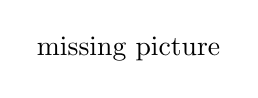
\begin{tikzpicture}
        \node {missing picture};
    \end{tikzpicture}
    \caption{Scalability results for the leader\_sync model}
    \label{fig:leader_results}
\end{figure}

\begin{figure}
    \centering
    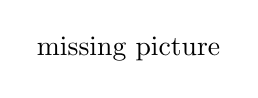
\begin{tikzpicture}
        \node {missing picture};
    \end{tikzpicture}
    \caption{Scalability results for the polling model}
    \label{fig:polling_results}
\end{figure}